\documentclass[11pt]{article}
\usepackage[utf8]{inputenc}
\usepackage[ngerman]{babel}

\usepackage{amsmath,amsthm,amssymb,amsfonts}

\usepackage{graphicx}
\graphicspath{{abb/}}
\usepackage{float}
\usepackage{tikz}

\usepackage{fancyhdr} % For headers and footers
\usepackage{geometry}
\usepackage{listings}
\usepackage{hyperref}
\hypersetup{
    linkcolor=blue,     
    urlcolor=cyan,
}

\geometry{
    a4paper, % Change this if you intend to print on a different paper size, such as letter paper.
    left=20mm,
    right=20mm,
    top=30mm,
    bottom=30mm,
}

\title{Kinematik in einer Raumrichtung - konstante Beschleunigung}
\author{Emil Staikov}
\date{19. Februar 2021}

\begin{document}
\maketitle
\section{Definition der Beschleunigung}
Die erste Erweiterung unserer Bewegungsbetrachtung bildet die Beschleunigung. Die Beschleunigung ist die Änderung der Geschwindigkeit in einem Zeitabschnitt, die Beschleunigung verhält sich zur Geschwindigkeit also genau wie die Geschwindigkeit zum Ort. Als Gleichung:
\begin{gather}
    a = \frac{\Delta v}{\Delta t} = \frac{v_2 - v_1}{t_2 - t_1}
\end{gather}
wobei $v_1$ die Geschwindigkeit am Zeitpunkt $t_1$ und $v_2$ die Geschwindigkeit am Zeitpunkt $t_2$ ist (als Wertepaare: $(t_1, v_1), (t_2, v_2)$). Streng genommen ist das die Definition der Durchschnittsbeschleunigung, die Momentanbeschleunigung finden wir, indem wir immer kleinere $\Delta t$ betrachten. Im Fall $a = const.$ sind Durchschnitts- und Momentanbeschleunigung stets gleich. 

\section{Bewegungsgleichungen für konstante Beschleunigung}
Aus der Definition der Beschleunigung finden wir als Ausdruck für die Geschwindigkeit in Abhängigkeit von der Zeit:
\begin{gather}
    \nonumber a = \frac{v_2 - v_1}{t_2 - t_1} = \frac{v(t)-v_0}{t-0} = \frac{v(t) - v_0}{t} \text{ (Wir setzen } t_1 = 0 \text{ und } t_2 = t \text{, folglich } v_1 = v_0 \text{ und } v_2 = v(t) \text{)} \\
    \Longleftrightarrow v(t) = at+v_0
\end{gather}
Die Geschwindigkeit wird damit durch eine lineare Funktion mit Anstieg $a$ beschrieben. \\
Um nun den Weg in Abhängigkeit von der Zeit zu bestimmen versuchen wir den Fall konstanter Beschleunigung auf die uns bekannte GGB zurückzuführen. Wenn wir die Geschwindigkeit über einem Zeitintervall $[0, t]$ betrachten, fällt uns auf, dass wir die gleiche Strecke zurücklegen würden, wenn wir uns über dem Intervall durchgängig mit der Durchschnittsgeschwindigkeit $\displaystyle v_{av} = \frac{v_0 + v(t)}{2}$ bewegen würden. Das liegt daran, dass die Fläche unter dem Geschwindigkeitsgraphen für die konstante Durchschnittsgeschwindigkeit gleich der Fläche unter dem Geschwindigkeitsgraphen für die lineare Momentangeschwindigkeit ist. Das kann man Elementargeometrisch beweisen (versucht es gerne mal). Bei der AG zur GGB haben wir festgestellt, dass die zurückgelegte Strecke der Fläche unter dem Graphen der Geschwindigkeit entspricht. 
\begin{figure}[H] 
    \centering
    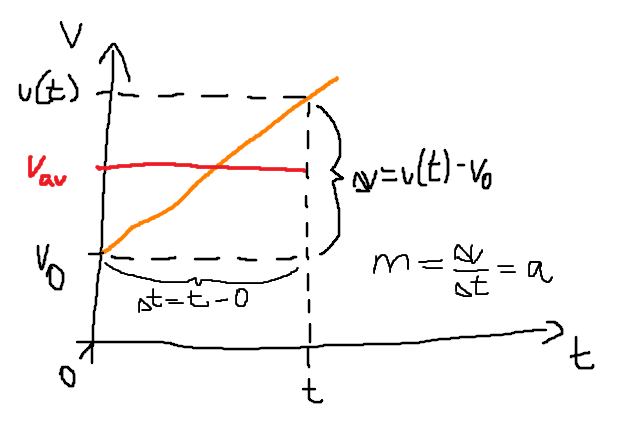
\includegraphics[width=0.6\textwidth]{v-t-diagramm-a-const.png}
    \caption{v-t-Diagramm bei konstanter Beschleunigung}
\end{figure} 
Durch einige Umformungen finden wir nun einen Ausdruck für den Ort in Abhängigkeit von der Zeit im Fall konstanter Beschleunigung: 
\begin{gather}
    \nonumber v_{av} = \frac{v_0 + v(t)}{2} = \frac{at + 2v_0}{2} = \frac{\Delta s}{\Delta t} = \frac{s(t)-s_0}{t-0} \text{ mit Definition der Geschwindigkeit und (2)} \\
    \Longleftrightarrow s(t) = \frac{a}{2}t^2 + v_0t + s_0
\end{gather}
$s(t)$ ist damit eine quadratische Funktion und wird grafisch durch eine Parabel beschrieben. Äquivalent zum Verhältnis von $v$ und $s$ bei der GGB findet man die Geschwindigkeit auch als Fläche unter dem Graphen der Beschleunigung wieder, zeichnet euch das für den Fall $a=const.$ mal auf um diesen Zusammenhang nachzuvollziehen. Zur Inspiration könnt ihr euch nochmal das Skript zur GGB anschauen. 

\section{Allgemeine grafische Interpretation der Beschleunigung}
Auch allgemein ist die Beschleunigung an einem Zeitpunkt stets gleich dem Anstieg der Geschwindigkeit an diesem Zeitpunkt. Was Anstieg allgemein bedeutet werden wir jedoch nicht behandeln, im Fall linearer Funktionen kennen wir diesen jedoch bereits (s. Abb. 1). Die Fläche unter dem Graphen der Beschleunigung entspricht stets der Geschwindigkeit. 
\end{document}